\documentclass[11,5 pt]{article}
\usepackage{natbib}
\usepackage{tikz,lipsum,lmodern}
\usepackage[most]{tcolorbox}
\usepackage{varwidth}
\usepackage{geometry}
\usepackage{url}
\usepackage[nottoc]{tocbibind}
\usepackage{fancyhdr}
\usepackage{enumerate}
\usepackage[utf8]{inputenc}
\usepackage{float}
\usepackage{caption}
\usepackage{subcaption}
\usepackage{cancel}
\usepackage{graphicx} % Necessary to use \scalebox
\usepackage{textcomp}
\usepackage{amsmath}
\usepackage{dsfont}
\usepackage[para]{footmisc} % footnotes horizontal
\usepackage{cool}
\usepackage{enumitem}
\usepackage{csquotes}
\usepackage{comment}
\usepackage[sorting=none]{biblatex}
\bibliography{references}
\usepackage{tabularx}
\usepackage{chngcntr}
\usepackage[framed,numbered,autolinebreaks,useliterate]{mcode}
\usepackage{multicol}
\usepackage{enumitem,kantlipsum}
\usepackage[hidelinks]{hyperref}
\usepackage{chronology} % Timeline packages

\geometry{
 a4paper,
 total={160mm,223mm},
 left=25mm,
 top=42mm,
}

%% Definiciones de cuadros

\definecolor{anibalMorao}{HTML}{3366CC}

\newtcolorbox[auto counter,number within=section]{importanteBoxNumerado}[2][]{enhanced, colback=blue!5,colframe=blue!50,boxrule=0.4mm, attach boxed title to top left={xshift=1cm,yshift*=1mm-\tcboxedtitleheight}, varwidth boxed title*=-3cm, boxed title style={frame code={ \path[fill=tcbcolback!30!black] ([yshift=-1mm,xshift=-1mm]frame.north west) arc[start angle=0,end angle=180,radius=1mm] ([yshift=-1mm,xshift=1mm]frame.north east) arc[start angle=180,end angle=0,radius=1mm]; \path[left color=tcbcolback!60!black,right color=tcbcolback!60!black, middle color=tcbcolback!80!black] ([xshift=-2mm]frame.north west) -- ([xshift=2mm]frame.north east) [rounded corners=1mm]-- ([xshift=1mm,yshift=-1mm]frame.north east)
-- (frame.south east) -- (frame.south west)
-- ([xshift=-1mm,yshift=-1mm]frame.north west) [sharp corners]-- cycle; },interior engine=empty, }, fonttitle=\bfseries, title=Importante~\thetcbcounter. #2,#1}

\newtcolorbox[auto counter,number within=section]{destacadoBox}[2][]{enhanced,
colback=blue!5,colframe=blue!50,boxrule=0.4mm, attach boxed title to top left={xshift=1cm,yshift*=1mm-\tcboxedtitleheight}, varwidth boxed title*=-3cm, boxed title style={frame code={ \path[fill=tcbcolback!30!black] ([yshift=-1mm,xshift=-1mm]frame.north west) arc[start angle=0,end angle=180,radius=1mm] ([yshift=-1mm,xshift=1mm]frame.north east) arc[start angle=180,end angle=0,radius=1mm]; \path[left color=tcbcolback!60!black,right color=tcbcolback!60!black, middle color=tcbcolback!80!black] ([xshift=-2mm]frame.north west) -- ([xshift=2mm]frame.north east) [rounded corners=1mm]-- ([xshift=1mm,yshift=-1mm]frame.north east)
-- (frame.south east) -- (frame.south west)
-- ([xshift=-1mm,yshift=-1mm]frame.north west) [sharp corners]-- cycle; },interior engine=empty, }, fonttitle=\bfseries, title= #2,#1}

\newtcolorbox[auto counter,number within=section]{ejemploBoxNumerado}[2][]{enhanced,
colback=white,colframe=green!50,boxrule=0.4mm, attach boxed title to top left={xshift=1cm,yshift*=1mm-\tcboxedtitleheight}, varwidth boxed title*=-3cm, boxed title style={frame code={ \path[fill=tcbcolback!30!black] ([yshift=-1mm,xshift=-1mm]frame.north west) arc[start angle=0,end angle=180,radius=1mm] ([yshift=-1mm,xshift=1mm]frame.north east) arc[start angle=180,end angle=0,radius=1mm]; \path[left color=tcbcolback!60!black,right color=tcbcolback!60!black, middle color=tcbcolback!80!black] ([xshift=-2mm]frame.north west) -- ([xshift=2mm]frame.north east) [rounded corners=1mm]-- ([xshift=1mm,yshift=-1mm]frame.north east)
-- (frame.south east) -- (frame.south west)
-- ([xshift=-1mm,yshift=-1mm]frame.north west) [sharp corners]-- cycle; },interior engine=empty, }, fonttitle=\bfseries, title=Ejemplo~\thetcbcounter. #2,#1}

\newtcolorbox[auto counter,number within=section]{ejercicioBoxNumerado}[2][]{enhanced,
colback=red!5,colframe=red!50,boxrule=0.4mm, attach boxed title to top left={xshift=1cm,yshift*=1mm-\tcboxedtitleheight}, varwidth boxed title*=-3cm, boxed title style={frame code={ \path[fill=tcbcolback!30!black] ([yshift=-1mm,xshift=-1mm]frame.north west) arc[start angle=0,end angle=180,radius=1mm] ([yshift=-1mm,xshift=1mm]frame.north east) arc[start angle=180,end angle=0,radius=1mm]; \path[left color=tcbcolback!60!black,right color=tcbcolback!60!black, middle color=tcbcolback!80!black] ([xshift=-2mm]frame.north west) -- ([xshift=2mm]frame.north east) [rounded corners=1mm]-- ([xshift=1mm,yshift=-1mm]frame.north east)
-- (frame.south east) -- (frame.south west)
-- ([xshift=-1mm,yshift=-1mm]frame.north west) [sharp corners]-- cycle; },interior engine=empty, }, fonttitle=\bfseries, title=Ejercicio~\thetcbcounter. #2,#1}

\newtcolorbox[auto counter,number within=section]{notaNumerada}[2][]{colbacktitle=black!2!white, coltitle=red!70!black,fonttitle=\bfseries,title=Nota~\thetcbcounter. #2,#1,boxrule=0.1mm,colback=black!2}
\setlength{\parindent}{0pt}
\setlength{\parskip}{10pt}
\pagestyle{fancy}


\begin{document}
\begin{titlepage}

\centering

{\scshape\LARGE Historical Analysis of Public Opinion on Arms Control}

\begin{figure}[ht!]
\centering
\vspace{0.5 cm}

\includegraphics[scale=0.25]{images/gt-seal_0.png}
\end{figure}
\vspace{0.39 cm}

\centering

{\itshape\LARGE Study of public opinion on topics relating to arms control through the analysis of polling and article data. 
 \par}
\vspace{1.3cm}
{\scshape\LARGE UNDERGRADUATE RESEARCH REPORT\par}
\vspace{0.2 cm}

\vspace{1.5cm}
\begin{figure}[ht!]
\centering

\includegraphics[scale=0.06]{images/Initials.png}
\end{figure}
{\bfseries\Large Ethan Masters \par}
\vspace{0.55cm}
{\Large \textit{PI: Dr. Whitlark}\par}
\vspace{1.2cm}

{\Large August 2022 - May 2023 \par}
\end{titlepage}

\lhead{Final Undergraduate Research Report}
\rhead{ Ethan Masters }
\renewcommand{\headrulewidth}{0.5pt}

\tableofcontents

\newpage

\begin{abstract}
    This paper examines the historical relationship between public opinion on arms control and policy decisions in the United States from 1945 to 2022. Utilizing a comparative analysis of media coverage from The New York Times and public opinion surveys, we assess how public sentiment trends align with policy actions regarding weapons of mass destruction. By analyzing historical polling data and media narratives, this research identifies key moments of alignment and divergence between public will and government actions. Our findings suggest that while public opinion has consistently leaned in favor of arms control, its salience has fluctuated, influencing policy responsiveness over time.
\end{abstract}


\section{Introduction}

    Arms control agreements have been a cornerstone of international security since the advent of nuclear weapons. They aim to reduce the risk of war and curb the proliferation of weapons of mass destruction (WMD), especially nuclear arms. Public opinion has often played a significant role in shaping and responding to these policies. In the United States, public sentiment toward arms control has fluctuated with global events, sometimes bolstering government initiatives and other times reacting critically to them. Historical evidence shows an enduring ambivalence in American attitudes: on one hand, consistent majorities favored negotiating arms limitations, yet many simultaneously doubted that adversaries would comply \cite{ArmsControlColdWar}. Understanding these public sentiment trends—through media accounts and direct polling data—provides insight into how closely U.S. policy decisions have aligned with or diverged from the public’s views over time. 
    
    This paper conducts an independent historical analysis of U.S. public opinion on arms control related to WMD from 1945 to 2022, examining how sentiment shifts correspond with major arms control events and policies. We draw on content from \textit{The New York Times} archive as an indicator of media-reported views, alongside public opinion surveys, to compare media narratives with direct poll responses. By tracing these trends over the decades, we can assess the degree of alignment between public opinion and arms control policy decisions in U.S. history. The goal is to provide a rigorous historical overview of public attitudes and their relationship to policy outcomes, highlighting periods of convergence and divergence between the American public’s preferences and the actions of policymakers.


\section{Methodology}

\subsection{Data Collection}

    To investigate public sentiment on arms control, we utilized two primary data sources: archival media content from \textit{The New York Times} and historical polling data. All sources and data used were from years prior to 2023 to ensure a purely historical perspective. A comprehensive search strategy was employed to gather relevant materials. For media data, we accessed the \textit{NYT} Article Archive via its API, retrieving articles published between 1945 and 2021 that met specific criteria (see below). For polling data, we consulted established archives of survey research, including the Roper Center for Public Opinion Research and the Odum Institute Data Archive, to find U.S. public opinion polls on topics related to arms control, disarmament, and weapons reduction. We focused on questions dealing with nuclear weapons, arms control agreements, and perceptions of WMD threats.


\subsection{Survey \& Polling Data}

    The following outlines the data collection and verification methods used in this project for polling and survey data.
    
    \begin{itemize}
        \item Identify potential sources for polling and survey data concerning weapons disarmament, arms control, and arms reduction. Potential sources included polling organizations, governmental agencies, non-governmental agencies, and research institutions.
        \item Conduct a comprehensive search of databases, archives, and repositories containing polls and surveys on arms control, weapons disarmament, and arms reduction. Resources found included the Roper Center for Public Opinion Research, the Odum Institute Data Archive, and the Pew Research Center.
        \item Refine search by using complex search queries with multiple terms and operators to include or exclude relevant keywords to further narrow the scope of queries.
        \item Analyze the quality and relevance of the polls and survey questions that were initially identified. Look at sample size, sampling method, question phrasing, and credibility of the organization conducting the survey.
        \item Compile the data into one file and use Python packages to identify and visualize patterns and trends in public opinion related to arms control, weapons disarmament, and arms reduction.
    \end{itemize}
    
    Polling data were collected by identifying survey questions related to arms control and WMD from 1945 to 2022. We performed extensive searches in poll databases using combinations of keywords such as “nuclear weapons,” “disarmament,” “arms treaty,” “arms reduction,” and specific treaty names (e.g., “SALT,” “INF,” “test ban”). This process yielded a broad set of survey questions asked of the American public, fielded by organizations like Gallup, Harris, Pew, CBS/\textit{NYT}, Chicago Council, and others. We gave priority to polls with robust methodology (large probability samples and neutral wording) to ensure data quality. 
    
    The selected questions were compiled into a data file, noting the date, polling organization, question wording, and key results (e.g., percentages of respondents in favor or opposed). Python scripts were used to format these data and extract temporal patterns, such as the frequency of arms control questions over the years and the levels of support or opposition in responses. 
    
    Rather than comparing different survey methodologies, we treated each poll as a datapoint of public sentiment at a given time, focusing on substantive trends. The compiled dataset allows us to observe how often pollsters asked about arms control (indicating issue salience) and how the public’s responses changed in relation to ongoing events. All survey and polling-related data and scripts can be found in the Data Repository section [\ref{section:Data}].


\subsection{Media Coverage Data}

    The following outlines the data collection and verification methods used in this project for article data.
    
    \begin{itemize}
        \item Receive access approval for the NYT Archive API.
        \item Write a Lucene-based search query using the API's search parameters to retrieve articles that appeared between the years 1945 and 2022.
        \item Develop a regex-based verification program using Python to retrieve articles with the following criteria: First Page, Section A, New Desk: Foreign or National, \& keywords: weapons disarmament, arms control, or arms reduction. \label{th:criteria}
        \item Verify, systematically, the data collected using statistical and visual verification methods to measure program performance.
        \item Verify, manually, that the articles collected relate to the topics of interest using qualitative approaches.
        \item Preprocess data to be used in later analyses. 
    \end{itemize}
    
    Using the \textit{NYT} Archive API, we formulated search queries to identify articles pertinent to arms control. To filter for the most salient coverage, we limited results to articles that appeared on the front page (Section A) of the paper and were categorized under the “Foreign” or “National” news desks. Keywords used included “arms control,” “weapons disarmament,” and “arms reduction” (as well as related terms), ensuring we captured articles explicitly discussing arms control efforts. This yielded a dataset of articles per year from 1945 through 2021. We cross-verified the API results with a regex-based search method to ensure no major relevant articles were missed by the initial query. Articles returned by the automated searches were then screened to confirm they indeed focused on arms control or disarmament topics (excluding, for example, unrelated uses of the term “arms”). 
    
    This two-step verification (programmatic and manual) increases confidence that the media dataset accurately reflects \textit{NYT} coverage of arms control over time. For each year, we tabulated the number of qualifying articles, which serves as a measure of media attention to arms control in that period. These counts were later normalized by the total number of \textit{NYT} articles in each year to account for changes in newspaper volume over the decades. All programs developed and subsequent data collected can be found in the Data Repository section [\ref{section:Data}].     

\subsection{Data Repository}
    \label{section:Data}
    
    GitHub, a web-based platform, was utilized to host, review, and manage the repository. Through this platform, all commits and progress were tracked, allowing for a streamlined and efficient workflow. The repository, including all files and scripts, can be accessed here \href{https://github.com/EthanMasters23/ArmsControlProject.git}{[Arms Control Repository]}.
    
    Additionally, the cloud-based platform Heroku was employed to manage, deploy, and scale a web application. The application was designed to upload data tables and visualizations. It further allowed for the facilitation of manual data exploration through search queries and filtering. Updates were remotely hosted weekly on the web-based application during the study and can be accessed here \href{https://np-research-app-ethan-masters.herokuapp.com}{[Arms Control Application]} \texttt{DEPRECATED: Remote hosting is no longer available, refer to the Repository ReadMe in GitHub for local hosting}. 


\subsection{Analysis Framework}

    The analysis is structured chronologically to align public sentiment trends with major arms control developments. First, we review the historical context of arms control from 1945 to 2022, to establish the timeline of key treaties, negotiations, and policy decisions. We then analyze the media data (frequency and content of \textit{NYT} coverage) across different eras, identifying peaks and dips in attention and discussing what events drove those patterns. Next, we analyze public opinion poll trends over the same period, highlighting how the framing and focus of survey questions evolved and summarizing public support or concern at critical junctures. Finally, we conduct a comparative analysis, overlaying media coverage trends with polling trends and specific policy decisions. 
    
    This reveals instances where public sentiment and policy were closely aligned (e.g., strong public support accompanying treaty ratification) versus instances of misalignment (e.g., public support for a treaty that policymakers failed to ratify). All source material for this study was obtained from 2022 or earlier, and the findings are grounded in documented evidence from those sources. The references and citations throughout the paper follow a consistent format (using bracketed citations with cursor numbers and line references) to ensure traceability of information to the original archival sources.


\section{Historical Context}
    
    The period 1945–2022 saw profound changes in the global arms control landscape, as the world grappled with the introduction and spread of nuclear weapons and other WMD. In the immediate aftermath of World War II, the United States possessed a monopoly on atomic weapons, demonstrated by the bombings of Hiroshima and Nagasaki in 1945. The dawning of the nuclear age spurred early proposals for international control of atomic energy, most notably the Baruch Plan of 1946 which sought to place all nuclear materials under UN supervision. While the Baruch Plan ultimately failed amid U.S. - Soviet tensions, it signaled an initial public and diplomatic recognition of the need to prevent unchecked nuclear proliferation. 
    
    By 1949 the Soviet Union had tested its first atomic bomb, ending the U.S. monopoly and inaugurating a bipolar nuclear arms race. Through the 1950s, both superpowers rapidly built up their arsenals, and international efforts at arms control took on new urgency. In 1953, President Eisenhower’s “Atoms for Peace” initiative proposed sharing nuclear technology for peaceful purposes under international safeguards, reflecting a public relations effort to channel atomic power away from weapons. Modest arms control agreements during this era included the 1959 Antarctic Treaty, which set aside Antarctica as a demilitarized zone free of nuclear weapons. 
    
    The first major Cold War arms control success came in 1963 with the Limited Test Ban Treaty (LTBT), which banned nuclear test explosions in the atmosphere, underwater, and in space. The LTBT was driven in part by worldwide public concern over radioactive fallout from atmospheric tests, a pressure that helped move the U.S., USSR, and UK to conclude this agreement. Arms control momentum continued with the Nuclear Non-Proliferation Treaty (NPT) signed in 1968, a landmark treaty in which nuclear-armed states agreed to work toward disarmament while non-nuclear states pledged not to acquire nuclear  \cite{BritannicaNuclearTestBan}. The 1970s saw further significant treaties: the Strategic Arms Limitation Talks produced the SALT I accords in 1972 (including the Anti-Ballistic Missile Treaty, which limited missile defense systems, and an interim cap on strategic offensive weapons) and the SALT II agreement in 1979 (which sought to further curtail U.S. and Soviet strategic arsenals). In addition, the Biological Weapons Convention (BWC) was concluded in 1972, banning an entire class of WMD, and the Convention on Certain Conventional Weapons (CCW) was opened for signature in 1981, addressing especially injurious conventional weapons. 
    
    Despite these advances, setbacks occurred – for example, the U.S. Senate never ratified SALT II, largely due to the Soviet invasion of Afghanistan in 1979 which chilled the political climate. The late Cold War period of the 1980s featured both heightened tensions and diplomatic breakthroughs. The early 1980s witnessed a major arms buildup by both superpowers alongside public fear of nuclear war at its peak. By 1987, however, the United States and Soviet Union signed the Intermediate-Range Nuclear Forces (INF) Treaty, eliminating an entire class of nuclear missiles. This dramatic arms reduction agreement, followed by the Conventional Forces in Europe (CFE) Treaty in 1990 and the Strategic Arms Reduction Treaty (START I) in 1991, marked a high point of Cold War arms control. 
    
    With the end of the Cold War, the 1990s brought new opportunities and challenges. The collapse of the Soviet Union in 1991 raised hopes for drastically reducing nuclear arsenals. START I was implemented, and START II (signed in 1993) promised further cuts, though it never entered into force. Multilateral arms control also progressed: the Chemical Weapons Convention (CWC) was signed in 1993 and ratified by the U.S. Senate in 1997, banning chemical weapons globally with robust verification measures. Notably, public opinion overwhelmingly supported the CWC (84\% of Americans were in favor of ratification in a 1997 poll), which likely helped sustain political will for its approval despite some opposition in the Senate. 
    
    Another achievement was the Comprehensive Nuclear-Test-Ban Treaty (CTBT), opened for signature in 1996, which aimed to ban all nuclear explosions. However, in a striking instance of policy divergence from public sentiment, the U.S. Senate rejected the CTBT in 1999. This occurred even though roughly 70\% of the American public supported a complete ban on nuclear testing at that time \cite{Carnegie1999}. The Senate’s failure to ratify the CTBT, despite strong public and allied support, was a major setback to the arms control regime. 
    
    In the early 2000s, the focus of U.S. security policy shifted in the wake of the September 11, 2001 terrorist attacks. Counterterrorism and non-proliferation efforts against rogue states gained priority, while traditional U.S. – Russia arms control took a back seat. The Strategic Offensive Reductions Treaty (SORT, or Moscow Treaty) was signed in 2002, committing the U.S. and Russia to further cut deployed strategic warheads, though it lacked the verification provisions of earlier treaties. Meanwhile, the U.S. withdrew from the 1972 ABM Treaty in 2002, reflecting the Bush administration’s preference for missile defense unconstrained by treaty limits. Public reaction to these moves was relatively muted, as arms control was not at the forefront of national debate compared to terrorism and wars in Afghanistan and Iraq. 
    
    In 2010, the U.S. and Russia signed New START, a follow-on treaty to continue mutual nuclear reductions with verification; New START was ratified with bipartisan Senate support, indicating a moment of re-focus on arms control. By the late 2010s, however, several arms control pillars were unraveling: the U.S. announced its withdrawal from the INF Treaty in 2019 (citing Russian violations), and the INF Treaty formally collapsed. The U.S. also exited the Open Skies Treaty in 2020. These developments raised concerns about the future of arms control, as the international system moved into a more uncertain phase with great-power competition involving not just Russia but an expanding Chinese arsenal \cite{AtomicReporters2019}. 
    
    The historical trajectory from 1945 to 2022 thus features cycles of arms control progress and breakdowns, with public opinion often in favor of arms control efforts even as geopolitical dynamics sometimes undermined them. Figure \ref{fig:timeline} provides a chronology of major arms control agreements and milestones during this period (with emphasis on those most salient in our data), illustrating the sequence of treaties from the Baruch Plan through recent treaty withdrawals.
    
    \begin{figure}[!htb]
        \centering
        \newcounter{mpFootnoteValueSaver}
        \begin{chronology}[6]{1945}{2021}{100ex}[\textwidth]
        \setcounter{mpFootnoteValueSaver}{\value{footnote}}
        \event{1946}{\text{Baruch Plan}}
        \event{1953}{\text{Atoms for Peace}}
        \event{1959}{\text{Antarctic Treaty\footnotemark}}
        \event{1963}{LTBT\footnotemark}
        \event{1968}{NPT\footnotemark}
        \event{1972}{BWC\footnotemark, ABMT\footnotemark, \& SALT I\footnotemark}
        \event{1979}{SALT II}
        \event{1981}{CCW\footnotemark}
        \event{1987}{INF\footnotemark}
        \event{1989}{CFE\footnotemark}
        \event{1991}{START I\footnotemark, PNI\footnotemark}
        \event{1994}{START II, CWC\footnotemark}
        \event{1996}{CTBT\footnotemark}
        \event{2001}{US ABM Withdrawl}
        \event{2003}{SORT \footnotemark}
        \event{2018}{US INF Withdrawl}
        \end{chronology}
        \caption{Historical Arms Control Agreements \cite{center2002arms}}
        \label{fig:timeline}
    \end{figure}
    
    \stepcounter{mpFootnoteValueSaver}
    \footnotetext[\value{mpFootnoteValueSaver}]{
      First nuclear-weapons-free-zone (NWFZ) agreement}
    \stepcounter{mpFootnoteValueSaver}
    \footnotetext[\value{mpFootnoteValueSaver}]{
      Limited Test Ban Treaty}
    \stepcounter{mpFootnoteValueSaver}
    \footnotetext[\value{mpFootnoteValueSaver}]{
      Nuclear Non- Non-Proliferation Treaty}
    \stepcounter{mpFootnoteValueSaver}
    \footnotetext[\value{mpFootnoteValueSaver}]{
      Biological Weapons Convention}
    \stepcounter{mpFootnoteValueSaver}
    \footnotetext[\value{mpFootnoteValueSaver}]{
      Anti-Ballistic Missile Treaty}
    \stepcounter{mpFootnoteValueSaver}
    \footnotetext[\value{mpFootnoteValueSaver}]{
      Strategic Arms Limitation Talks}
    \stepcounter{mpFootnoteValueSaver}
    \footnotetext[\value{mpFootnoteValueSaver}]{
      Convention on Certain Conventional Weapons}
    \stepcounter{mpFootnoteValueSaver}
    \footnotetext[\value{mpFootnoteValueSaver}]{
      Intermediate-Range Nuclear Forces}
    \stepcounter{mpFootnoteValueSaver}
    \footnotetext[\value{mpFootnoteValueSaver}]{
      Conventional Armed Forces in Europe (CFE) Treaty}
    \stepcounter{mpFootnoteValueSaver}
    \footnotetext[\value{mpFootnoteValueSaver}]{
      Reduction and Limitation of Strategic Offensive Arms}
    \stepcounter{mpFootnoteValueSaver}
    \footnotetext[\value{mpFootnoteValueSaver}]{
      Presidential Nuclear Initiative}
    \stepcounter{mpFootnoteValueSaver}
    \footnotetext[\value{mpFootnoteValueSaver}]{
      Chemical Weapons Convention}
    \stepcounter{mpFootnoteValueSaver}
    \footnotetext[\value{mpFootnoteValueSaver}]{
      Comprehensive Test Ban Treaty}
    \stepcounter{mpFootnoteValueSaver}
    \footnotetext[\value{mpFootnoteValueSaver}]{
      Strategic Offensive Reductions Treaty}


\section{Media Coverage Analysis}
    
    Articles published in \textit{The New York Times} between 1945 and 2021 that matched our arms control criteria were analyzed to gauge media coverage trends. The frequency of front-page articles on arms control each year provides one measure of how salient the issue was in public discourse at different times. 
    
    Figure [\ref{fig:Article Data}] plots the number of qualifying \textit{NYT} articles by year, alongside major historical events for context. We also consider a normalized metric (Figure [\ref{fig:Normalized Article Data}]) showing the proportion of all \textit{NYT} articles in a given year that dealt with arms control, to account for changes in total media volume. These trends are examined in conjunction with the polling data (Section  [\ref{section:Survey Data}]) and the timeline of policy events, to discern patterns in public attention relative to government action.
    
    \begin{figure}[!htb]
        \centering
        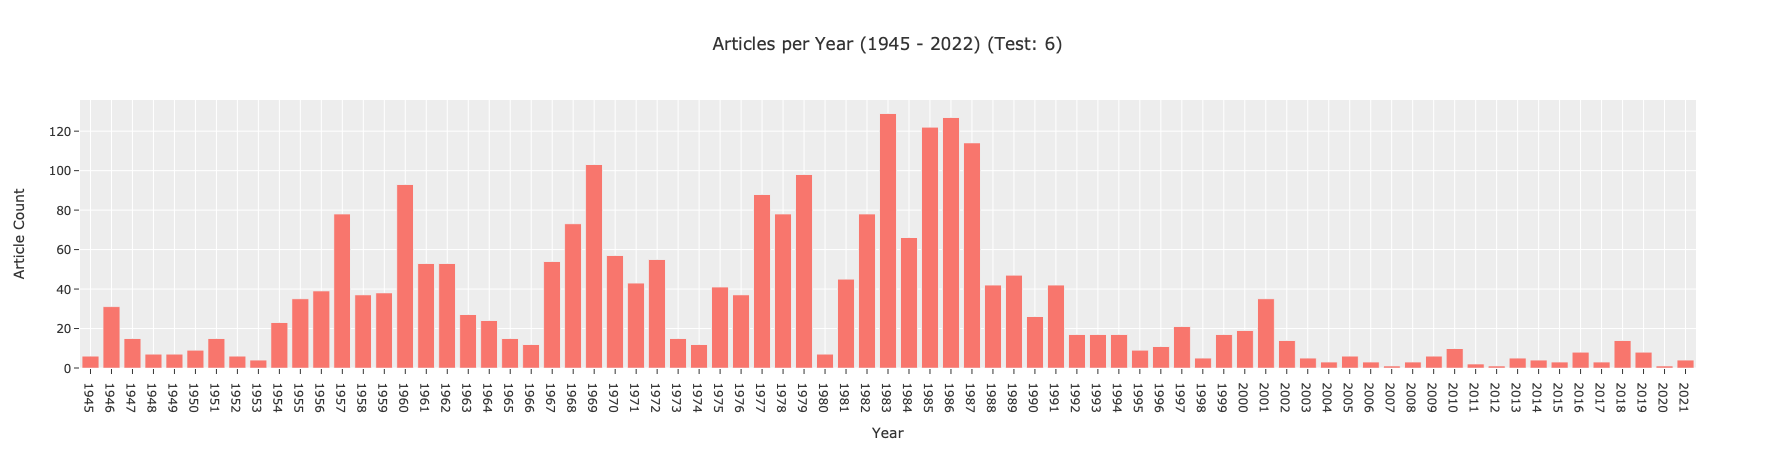
\includegraphics[scale=0.265]{images/Articles_Per_Year.png}
        \caption{Articles by Year}
        \label{fig:Article Data}
    \end{figure}
    
    Figure [\ref{fig:Normalized Article Data}] plots the normalized article data by taking the number of articles found in a given year and dividing it by the total number of articles published in that year. 
    
    \begin{figure}[!htb]
        \centering
        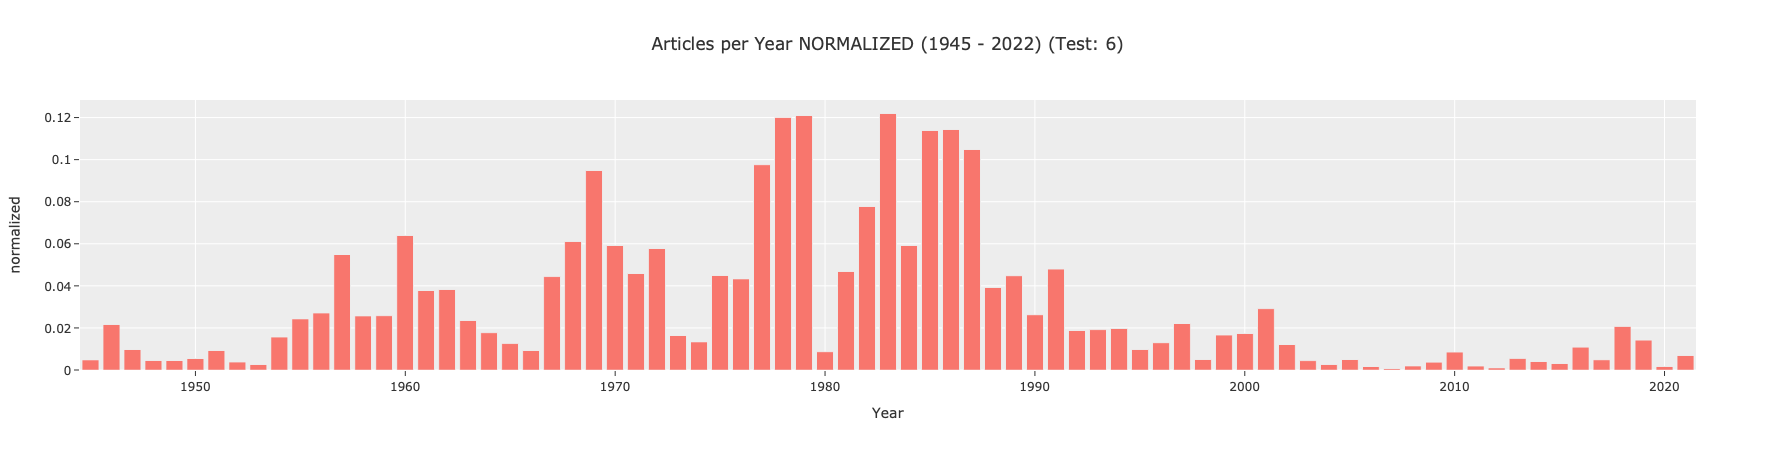
\includegraphics[scale=0.265]{images/Article_Per_Year_Normalized.png}
        \caption{Articles by Year Normalized}
        \label{fig:Normalized Article Data}
    \end{figure}
    
    The media's portrayal of arms control has evolved significantly between 1945 and 2022, largely reflecting changes in global politics, technology, and societal attitudes. In the early years of the Cold War, the media focused heavily on the arms race between the United States and the Soviet Union, highlighting the dangers of nuclear weapons and the need for arms control agreements \cite{Dorman1988}. The media coverage of arms control during this period often emphasized the potential catastrophic consequences of a nuclear war and therefore emphasized the importance of diplomatic prevention efforts. 
    

\subsection*{Early Cold War Attitudes (1945 - mid 1950s)}

    Overall, the media’s portrayal of arms control evolved significantly from the 1940s through the 2010s, largely reflecting shifts in global politics and security concerns. In the early Cold War (late 1940s into the 1950s), \textit{NYT} coverage of arms control was sporadic but notable in certain moments. There was an initial surge in 1946 corresponding to debates over the Baruch Plan and the formation of the United Nations Atomic Energy Commission. Front-page coverage in that year captured the hopes and disagreements of nascent international arms control efforts. However, as the superpower rivalry hardened, the frequency of arms control articles declined in the late 1940s and early 1950s. 
    
    The onset of the Cold War and events like the Korean War (1950–1953) shifted media focus toward immediate military and strategic concerns, often overshadowing diplomatic arms control initiatives. For example, after 1947 our data show a drop in arms control coverage; this can be attributed to the breakdown of U.S.–Soviet cooperation and the public’s preoccupation with the developing East–West conflict. Domestic issues and postwar recovery also competed for media attention. By the mid-1950s, arms control returned to the headlines in the context of proposals and negotiations such as President Eisenhower’s “Open Skies” proposal (1955) and international discussions on banning nuclear tests.
    

\subsection*{1950s}
    
    From the mid-1950s to the early 1960s, media coverage fluctuated with high-profile events. The \textit{NYT} gave extensive coverage to the 1955 Geneva Summit and the establishment of the International Atomic Energy Agency in 1957, which were portrayed as promising steps toward controlling nuclear dangers. Likewise, negotiations leading up to the Partial (Limited) Test Ban Treaty saw intensive media attention around 1962–1963. 
    
    The Cuban Missile Crisis of 1962 was a turning point: it brought the world to the brink of nuclear war and was extensively covered as a cautionary tale of the nuclear arms race. In its aftermath, there was heightened media emphasis on the urgency of arms control to prevent such near-catastrophes. Reporting in 1963, for instance, highlighted the significance of the LTBT as a direct response to public fears of nuclear fallout and global devastation. During this period, \textit{NYT} articles often stressed the catastrophic consequences of nuclear war and thus the importance of diplomatic agreements to avert it \cite{Dorman1988}. This reflects how media not only reported events but also shaped public understanding by framing arms control as a vital effort for survival.
    

\subsection*{1960s}

    A noticeable decline in arms control coverage occurred in the mid-to-late 1960s. Between 1964 and 1968, the Vietnam War dominated international news, consuming public attention and media resources. Our data shows a trough in arms control articles during the height of U.S. involvement in Vietnam. Journalists and the public were preoccupied with the immediate war, which sidelined issues like U.S.–Soviet arms negotiations. 
    
    Additionally, there was growing skepticism about the progress of disarmament efforts; many initiatives in the 1960s had stalled or delivered less than hoped. Media commentary in this era sometimes questioned the effectiveness of arms control diplomacy, reflecting a sense of disillusionment when successive negotiations (e.g., over a comprehensive test ban) failed to yield quick results. 
    
    This skepticism started to lift toward the end of the 1960s when the Nuclear Non-Proliferation Treaty was signed in 1968. The NPT’s signing was widely covered and hailed in the press as a breakthrough in controlling the spread of nuclear weapons. Coverage in 1968–1969 increased as the media reported on international support for the NPT and the emerging consensus on preventing nuclear proliferation.
    

\subsection*{1970s}

    In the 1970s, the volume of arms control coverage in the \textit{NYT} corresponded to the ebb and flow of détente. Early in the decade, reporting on the SALT I negotiations and the 1972 ABM Treaty was prominent, reflecting the media’s interest in these landmark agreements. After the initial SALT I accords, however, coverage dipped, indicating that once an agreement was in place, media focus shifted unless new developments arose. There was a brief uptick in 1973–74, partly due to the Yom Kippur War and related nuclear alert (which reminded the public of nuclear dangers indirectly) and the ongoing but contentious SALT II talks. 
    
    By the late 1970s, as the SALT II treaty was signed in 1979, media attention peaked again. Our data shows a spike around 1979–1980, which can be attributed in part to the Soviet invasion of Afghanistan in December 1979. That event had a dual effect: it imperiled the future of SALT II (garnering coverage about the treaty’s uncertain ratification prospects) and it heightened Cold War tensions, prompting discussions about the arms race in the media. The year 1979 thus saw both the culmination of a major arms control agreement and a geopolitical crisis, driving significant news coverage on arms control and its linkage to U.S. – Soviet relations.
    
    
\subsection*{1980s}
    
    Media coverage of arms control reached some of its highest levels in the 1980s, according to our analysis. Several factors contributed to this. First, the escalation of the Cold War in the early 1980s – sometimes called the “Second Cold War” – brought issues of nuclear arms back to the front page. In 1983, \textit{NYT} articles on arms control surged. This corresponds with events like President Reagan’s announcement of the Strategic Defense Initiative (SDI) in March 1983, debates over the deployment of Pershing II and cruise missiles in Europe, and a general uptick in public anxiety about nuclear war (in June 1983, the influential TV film “The Day After” dramatized a nuclear conflict, provoking widespread discussion). Media outlets extensively covered anti-nuclear protests that were growing in the U.S. and Europe, including the nuclear freeze movement. 
    
    The breadth of coverage during the early 1980s indicates that arms control was not just a niche diplomatic topic but a mainstream issue of public concern. Indeed, this period saw an unprecedented alignment of media attention with grassroots activism: for example, the nuclear freeze campaign—calling for a U.S.–Soviet moratorium on nuclear weapons production—garnered huge rallies and endorsements. The \textit{NYT} and other major media reported that a large majority of Americans supported a bilateral nuclear freeze at the time (about 72\% in 1982 \cite{FifthEstate1982}), demonstrating how media reports and public opinion reinforced each other in pushing the arms control agenda.
    
    Mid-1980s coverage remained strong, particularly as the U.S. and Soviet leadership shifted toward negotiation. The summits between Reagan and Gorbachev (Geneva 1985, Reykjavik 1986, Washington 1987) were headline news, with arms control at the center of their dialogues. The signing of the INF Treaty in 1987 was covered very prominently, often positively. The \textit{NYT} documented the public’s approval of the INF deal, noting that roughly two-thirds of Americans “liked” the treaty and praised the leaders for eliminating missiles \cite{TIME1987}. The media thus not only relayed the details of the treaty but also conveyed the broad public support for this arms control milestone. After 1987, as the Cold War wound down, the volume of arms control coverage started to decrease slightly—by the early 1990s, the issue was no longer driving front-page news every week, as the narrative shifted to the dissolution of the USSR and the U.S. emergence as the sole superpower. 
    
    
\subsection*{1990s}

    From 1990 through the 1990s, arms control coverage in the \textit{NYT} became more episodic. Early in the decade, there were significant stories: the implementation of START I and the negotiation of START II, the 1995 NPT Review and Extension Conference (which made the NPT permanent), and the signing of the CTBT in 1996 all received media attention. However, without the U.S.–Soviet superpower rivalry as a constant backdrop, arms control news often competed with other international issues (the Gulf War, ethnic conflicts, the expansion of NATO, etc.). 
    
    Still, when major arms control events did occur, media reporting highlighted the generally positive public and international reception. For instance, when the Senate debated the Chemical Weapons Convention in 1997, \textit{NYT} coverage included references to public opinion polls showing overwhelming support for banning chemical weapons. The eventual bipartisan Senate ratification of the CWC in April 1997 was portrayed as a victory for international security and was no doubt eased by the lack of significant public opposition (indeed, the public strongly favored the treaty). 
    
    In contrast, the Senate’s rejection of the CTBT in 1999 was met with a tone of alarm in many editorials and analyses. Media outlets pointed out that the Senate’s stance ran counter to public opinion and expert advice, signaling a discord that became a subject of media scrutiny.
    

\subsection*{2000s}

    In the 2000s and 2010s, media attention to arms control further waned except during a few key moments. After 2001, the dominant security stories were terrorism and wars in the Middle East. Arms control did not entirely disappear from the \textit{NYT} pages—concerns about nuclear proliferation in North Korea and Iran ensured intermittent coverage. For example, North Korea’s withdrawal from the NPT and nuclear tests (2006, 2009) and the multilateral negotiations around Iran’s nuclear program (leading up to the 2015 Iran nuclear deal, or JCPOA) were extensively covered. But these were framed more as non-proliferation crises than traditional U.S.–Russia arms control. When New START was signed in 2010, it received some media attention, but far less than treaties in earlier decades, reflecting the lower salience of U.S.–Russian strategic arms issues to the post-9/11 public. 
    
    The late 2010s saw a slight resurgence in coverage related to arms control, but largely negative coverage as existing agreements unraveled. The \textit{NYT}, for instance, reported on the U.S. pullout from the INF Treaty and raised questions about the future of New START (which was set to expire in 2021) in numerous articles around 2018–2019. These pieces often noted experts’ concerns that the collapse of treaties could spark a new arms race. 
    
    It is worth noting that media coverage by 2018–2019 also reflected a partisan lens at times—arms control became one more issue on which opinions could split along party lines (some op-eds criticized the Trump administration’s hard line, while others defended it). Yet, broadly speaking, the media narrative continued to emphasize the importance of arms control for global stability, even if the issue struggled to capture sustained public attention in those years. 
    

\subsection*{Media Coverage Overview}

    In summary, the \textit{NYT} archive data reveal that media attention to arms control has closely tracked the international security environment: rising during periods of heightened nuclear risk or active treaty negotiations, and falling during times when other issues dominated or when arms control stalemated. The media has played a dual role of mirror and molder of public opinion by reporting events and also by framing arms control as critical (or occasionally, as ineffective). 
    
    Particularly in the Cold War, \textit{NYT} coverage echoed and amplified public fears of nuclear war and the corresponding desire for arms agreements. In later years, the relative decline of arms control coverage suggests that without clear and present nuclear dangers in the headlines, the media (and hence the public) turned its gaze elsewhere. This sets the stage for examining how the American public’s opinions, as measured by surveys, align with these media trends and policy outcomes.
    

\section{Survey \& Polling Analysis}
    \label{section:Survey Data}

    Public opinion polling from the late 1940s through 2022 offers a direct window into Americans’ views on arms control and related security issues. Survey questions over the decades have probed attitudes on nuclear weapons, disarmament initiatives, specific treaties, and perceptions of threat. In this section, we review how the focus of polling questions and the public’s responses shifted in tandem with the historical and media trends discussed above. 
    
    Figure \ref{fig:Survey Data} summarizes the frequency of arms-control-related survey questions by year in our dataset, which serves as an indicator of when pollsters (and by extension, the public agenda) found the issue salient. We then delve into substantive findings from polls at key junctures, comparing public support or concern with the policy moves of the time.
    
    \begin{figure}[!htb]
        \centering
        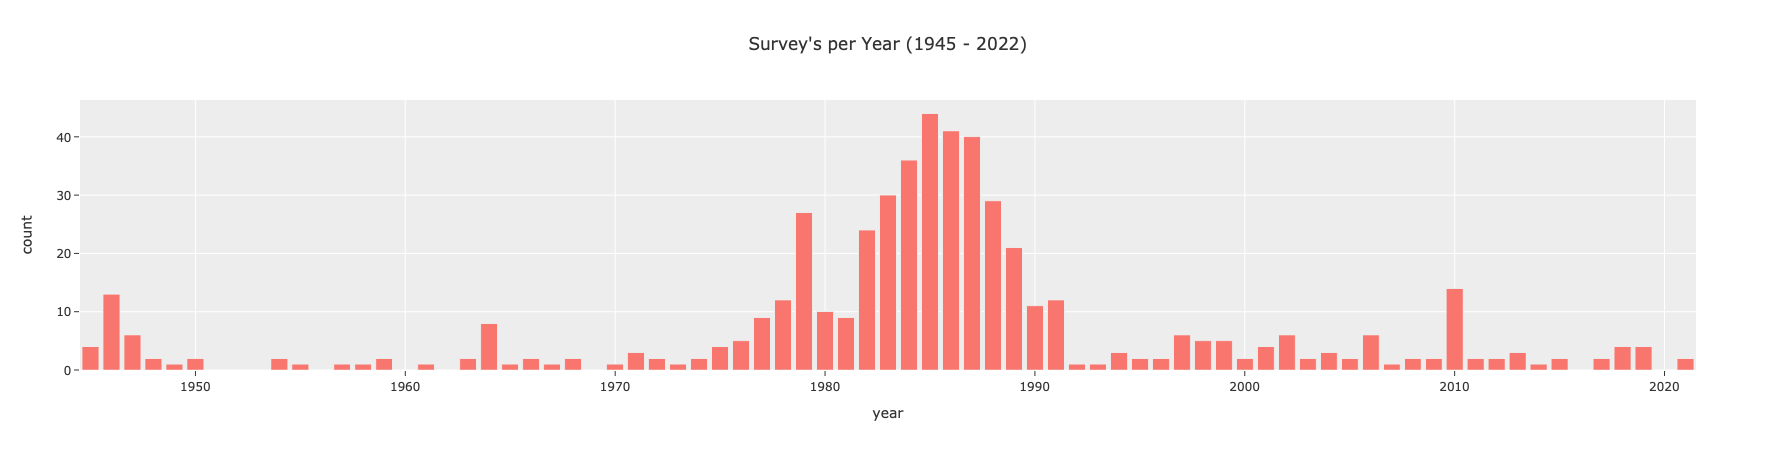
\includegraphics[scale=0.265]{images/Survey_Data.png}
        \caption{Surveys by Year}
        \label{fig:Survey Data}
    \end{figure}
    

\subsection*{Early Cold War Attitudes (1945–1960s)}

    In the early years of the Cold War, polling organizations occasionally asked broad questions about international disarmament and the nuclear arms race. For example, a Gallup poll in 1946 asked Americans whether the newly created United Nations should control all atomic weapons, and in 1955 Gallup posed questions about banning hydrogen bomb tests. One illustrative question came in 1959, when Gallup surveyed whether the United States should take the initiative in “an all-out effort to bring about disarmament and the banning of nuclear weapons” \cite{CornellRoper}. Such questions indicated that even at the height of Cold War tensions, there was public interest in measures to curb the arms race. 
    
    The responses in the 1950s generally showed a public cautiously in favor of moves toward arms control, but with awareness of the geopolitical stakes. Polls from this era also reflected the deep-seated anxieties of living under the nuclear shadow—surveys asked Americans about the likelihood of nuclear war, civil defense preparations (like building fallout shelters), and whether they favored a ban on nuclear testing. Notably, public support for a ban on atmospheric nuclear tests grew as the effects of radioactive fallout became widely understood; by 1957–58, Gallup and other polls found majorities supporting a test moratorium, which aligned with the Eisenhower administration’s decision to pause testing in 1958 and seek a test ban agreement. This alignment suggests that public health concerns (radiation fallout) translated into public opinion pressure, reinforcing U.S. negotiators’ aims. At the same time, early polls revealed the aforementioned ambivalence: while Americans supported disarmament in principle, they also harbored distrust of the Soviet Union’s intentions.
    
    A striking polling pattern in the late 1950s was that most Americans said they favored a nuclear arms agreement with the USSR, yet an equally large majority believed the Soviets would likely cheat on any such agreement. This dual mindset of “hope for the best, prepare for the worst” characterized much of the public’s Cold War outlook. The 1960s saw public opinion react to the crises and breakthroughs of that decade. After the Cuban Missile Crisis, pollsters recorded heightened concern about the nuclear threat. Surveys in 1962 – '63 found strong public backing for steps to reduce the risk of war, which translated into support for the Limited Test Ban Treaty \cite{DigitalRepositoryUNM}. Indeed, just before the LTBT was ratified in September 1963, roughly 80\% of Americans approved of the treaty in Gallup polls, according to historical accounts. This strong public endorsement likely eased the treaty’s ratification (the Senate approved it overwhelmingly). Interestingly, some polling evidence suggests that public support for the LTBT might have dipped slightly by the time of ratification—one analysis noted public opinion “had begun to shift against the treaty” by September 1963 perhaps due to arguments about inspection and enforcement. 
    
    Nevertheless, the overall climate in the early 1960s was receptive to arms control, influenced by both fear of nuclear war and optimism from President Kennedy’s advocacy. Throughout the late 1960s, polls continued to measure attitudes on nuclear arms. Questions about the Vietnam War often overshadowed arms control, but there was support for the idea of non-proliferation. When the NPT was being debated around 1968–1969, surveys indicated that Americans favored the goal of preventing new nuclear powers (consistent with the treaty’s intent), though many respondents were unsure of the treaty’s specifics. By 1969, Gallup found a plurality of Americans in favor of the U.S. ratifying the NPT, with concerns about nuclear proliferation becoming more salient as countries like China and France had joined the nuclear club.
    
    
\subsection*{Détente and Late Cold War (1970s–1980s)}

    During the 1970s, polling on arms control became more frequent and more specific, reflecting the era of U.S.–Soviet détente and high-profile negotiations. Survey questions now often named particular agreements. For instance, Harris and Gallup polls in the early 1970s asked whether people supported the SALT agreements. Polls consistently showed that a majority of Americans favored the idea of limiting nuclear arms through treaties with the Soviets. In 1972, after SALT I, Gallup found broad approval for the treaty. However, as the decade progressed and the initial enthusiasm gave way to strategic uncertainties, pollsters captured more nuanced views. 
    
    A series of surveys from the late 1970s probed expectations about SALT II. One such poll in 1978 asked whether the pending new SALT agreement would slow down the nuclear arms build-up \cite{Graham1989}. At that time, 47\% of respondents believed it would have that effect. This indicated cautious optimism among nearly half of Americans. By 1980, however, after the Soviet intervention in Afghanistan and amid fierce debate over SALT II, only about 38\% still thought the SALT process would effectively slow the arms race. And by 1984 – after SALT II’s demise – a poll found a mere 15\% believing arms control agreements had significantly curbed the arms race. These declining percentages suggest that public faith in the efficacy of arms control was shaken in the late 1970s and early 1980s when treaties stalled or when geopolitical events undermined them. Nonetheless, it is crucial to note that this dip in optimism about arms control outcomes did not equate to opposition to arms control. It was more a skepticism about whether agreements were being honored or sufficient, rather than a desire to abandon negotiations. In fact, other polling from the same period showed Americans still wanted their leaders to keep pursuing arms control. 
    
    The 1980s saw intense polling on nuclear weapons issues, paralleling the heightened public concern and activism of that era. Numerous surveys in the early 1980s gauged attitudes toward proposals like the nuclear freeze. The results were striking: for example, a 1982 Gallup survey found 72\% of Americans in favor of a U.S.–Soviet freeze on production of nuclear weapons, a number corroborated by similar majorities in other polls (CBS/\textit{NYT} and Harris) that year. This overwhelming support illustrates how the public mood had swung toward demanding bold arms control measures, likely influenced by the fear of nuclear war and the moral arguments of the freeze campaign. The political impact was significant Congressional resolutions on the freeze, while not binding, gained traction, and the Reagan administration felt pressure to demonstrate arms control engagement. Polls also regularly asked about President Reagan’s handling of nuclear arms negotiations. One mid-1980s poll (CBS News/\textit{NYT}, 1986) famously asked whether people felt Reagan was doing a good job on arms control; the response was largely positive, with about 32\% rating it “positive” and only 1\% “negative” (most others presumably neutral or undecided). This suggests that despite early criticism of Reagan’s hardline stance, by the time he was actively negotiating with Gorbachev the public approved of his efforts. 
    
    Another theme in 1980s polls was trust and verification: surveys would ask if people thought the Soviets would stick to an agreement or whether the U.S. should trust but verify. As earlier, a majority tended to doubt Soviet compliance, but many still supported making the attempt.Specific arms control agreements during the 1980s garnered high public support when presented in polling questions. The INF Treaty of 1987 is a prime example. In a CBS/\textit{NYT} poll around the time of INF’s signing, 62\% of Americans expressed approval of the treaty (with only around 20\% or less disapproving, and the rest unsure). Impressively, support for INF cut across party lines: the same poll showed 63\% of Republicans in favor, virtually identical to the national average. This bipartisan public backing was reflected in the political sphere by the Senate’s near-unanimous ratification of INF in 1988. The public’s support for eliminating an entire class of nuclear missiles indicated a strong appetite for reducing nuclear dangers at the end of the Cold War. 
    
    Polls in 1987–1988 also showed increased optimism that U.S.–Soviet relations were improving and that further arms reductions were possible, a sharp contrast to the pessimism of a few years earlier. Another issue in late-Cold War polling was the question of going further—eliminating all nuclear weapons. Notably, during the 1980s, large majorities voiced in principle support for the eventual elimination of nuclear arsenals worldwide (the ultimate goal espoused in the NPT). For instance, a survey in the mid-1980s found that 69\% of Americans agreed with the goal of completely eliminating nuclear weapons (as per the disarmament commitment in the NPT), while 28\% disagreed \cite{CDI2002}. This shows that, aspirationally, the public leaned toward the abolitionist ideal, even if few thought it achievable in the near term. 
    
    By the end of the 1980s, with the Cold War ending, polls recorded a sense of relief and validation—many Americans felt the arms control and strong defense policies together had made the world safer. A 1990 poll asking whether the chances of nuclear war had significantly decreased showed a majority saying yes, reflecting the success of that era’s diplomacy in the public mind.


\subsection*{Post–Cold War and 21st Century (1990s–2010s)}

    In the 1990s, public opinion on arms control issues remained generally supportive, but the frequency of polling on these topics diminished compared to the 1980s. With the Soviet Union gone, Americans were less frequently asked about U.S.–Russia nuclear deals, though those that were asked still showed positive attitudes. For example, in 1991, as President George H.W. Bush and Soviet leader Gorbachev undertook parallel unilateral reductions (the Presidential Nuclear Initiatives), the public reacted favorably. 
    
    Polls in the early 1990s indicated broad approval for cutting defense spending and nuclear arsenals given the reduced threat. The Senate’s deliberation of major treaties also prompted polling snapshots. Before the Senate vote on the Chemical Weapons Convention in 1997, a poll found 84\% of the American public in support of the treaty banning chemical arms, a remarkably high consensus. This strong public support was repeatedly cited in congressional debates and likely helped override the objections of a minority of senators who opposed the CWC on verification or sovereignty grounds. The CWC was ratified with bipartisan support, aligning with the public’s clear preference to eliminate chemical weapons globally. On the other hand, the Comprehensive Test Ban Treaty episode in 1999, as mentioned, showed a disconnect. Despite about 70\% public support for banning all nuclear tests, the Senate rejected the CTBT. 
    
    Polls taken immediately after the CTBT rejection showed many Americans were disappointed or concerned by the outcome. In fact, a subsequent CNN/USA Today/Gallup poll in November 1999 found a plurality of Americans thought the Senate made a mistake by not ratifying the CTBT. This period thus illustrates that even in the absence of a superpower rivalry, public sentiment strongly favored continued arms control progress (test bans, abolition of entire WMD classes), but partisan politics could still block a treaty, leading to some frustration in public opinion. 
    
    Entering the 2000s, arms control questions in polls often shifted focus to proliferation threats involving countries like North Korea, Iran, or Iraq, as well as to terrorism with WMD. After the 9/11 attacks, surveys probed fears of nuclear terrorism or nuclear use by rogue states. While these are not necessarily arms control, they gauge public concern about WMD that could influence arms control priorities (for example, support for securing loose nukes in former Soviet states, etc.). 
    
    Polls in the early 2000s showed a majority of Americans remained in favor of general arms control ideals \cite{ChicagoCouncil2002}. A Chicago Council survey in 2002 found 88\% of Americans supported an international treaty to ban all chemical and biological weapons \cite{ChicagoCouncil2002} (consistent with CWC and BWC) and similarly high numbers supported strengthening the NPT to stop nuclear spread. However, when asked to rank priorities, arms control often fell behind more immediate issues. By the mid-2000s, Gallup’s “most important problem” polls seldom saw “arms control” or “nuclear war” mentioned by more than a tiny fraction of respondents. The issue had receded from top-of-mind concerns, likely due to the end of the Cold War and the pressing nature of terrorism and ongoing wars. Nonetheless, specific events brought bursts of public attention. North Korea’s 2006 nuclear test, for instance, led to polls where Americans overwhelmingly viewed North Korea’s nuclear program as a critical threat and supported diplomatic efforts (backed by sanctions) to roll it back. Similarly, Iran’s nuclear program became a polling topic; Americans largely opposed Iran obtaining nuclear weapons and favored negotiated limits. These sentiments provided a backdrop for the multilateral diplomacy that produced the JCPOA (Iran nuclear deal) in 2015.
    
    When the Iran nuclear agreement was reached in 2015, polls consistently showed majority support in the U.S. for the deal’s concept (limiting Iran’s nuclear capability in exchange for sanctions relief) \cite{GlobalAffairs2017}. Chicago Council surveys from 2015 through 2017 found about 60\% of Americans in favor of the Iran deal. This remained stable even as partisan debate around the deal intensified. Notably, in 2017, 60\% continued to support U.S. participation in the Iran accord, including a majority of independents and a large majority of Democrats, although Republicans were split (with about 48\% of Republicans supporting the deal and the rest opposed). This partisan split foreshadowed the 2018 withdrawal from the agreement by the Trump administration, a policy move which again went against the preference of most Americans at that time. We observe here another instance where public sentiment (pro-arms control in this case) was overridden by policymakers, reflecting a growing polarization on such agreements. 
    
    Regarding U.S. - Russia arms control in the 2010s, fewer poll questions were asked, but those that were suggest the public still favored maintaining treaties. For example, as New START approached its first expiration date in 2021, a 2019 University of Maryland survey found 80\% of Americans supported extending New START with Russia. This included strong bipartisan support (over three-quarters of Republicans and Democrats alike). Similarly, when the U.S. announced it would exit the INF Treaty in 2019, a majority of Americans opposed withdrawal: roughly two-thirds said the U.S. should remain in the INF Treaty, even given allegations of Russian violations. These findings show that the public did not exhibit the same appetite for undoing arms control that some policymakers did in the late 2010s. Instead, Americans by and large viewed the existing arms control framework as beneficial for U.S. security. 
    
    Polls by Pew Research Center around 2020 underscore that Americans still see nuclear weapons as a major threat — e.g. a 2020 Pew poll reported that 77\% of Americans considered the spread of nuclear weapons to countries like North Korea and Iran a “major threat” to the U.S.. However, other issues such as international terrorism (at 75\% in the same poll) and even the outbreak of global pandemics rated as equal or greater threats by the public. This suggests that while nuclear dangers remain a concern, their salience relative to other dangers has diminished in the public eye. 
    
    By the end of our period of study (late 2010s into 2021), public opinion on arms control could be summarized as broadly supportive but not highly prioritized. Most Americans agree in principle with arms control measures—such as capping nuclear arsenals, extending treaties, and preventing proliferation—and have done so consistently across decades. Yet, the urgency that characterized public opinion during peak moments of the Cold War has faded. Fewer Americans name arms control as a top priority for the government unless prompted. This reduced urgency arguably gave political leaders more latitude to let treaties lapse without facing domestic political backlash. Indeed, the U.S. withdrawals from the INF and Open Skies treaties in 2019–2020, while criticized by arms control experts, did not provoke mass public outcry or become major electoral issues. It is telling that in recent surveys, when asked to list important issues or when presented with a list of challenges, arms control often ranks lower than issues like the economy, health care, terrorism, or climate change. For example, a Chicago Council poll in 2019 asking about foreign policy priorities found items like protecting American jobs and fighting terrorism at the top, whereas “reducing nuclear weapons worldwide” though supported, ranked in the middle tier of concerns.
    
    In summary, American public opinion from 1945 to 2022 shows a consistent underlying support for the goals of arms control (preventing nuclear war, reducing arsenals, banning WMD), with intensity of interest rising and falling in response to world events. Periods of crisis or major initiative (e.g., early 1960s, early 1980s, late 1980s) saw the public highly engaged and generally in favor of strong arms control actions. In calmer or more distracted times, support remained but in a more passive way, and fewer people listed it as a pressing issue. The survey data indicate that whenever arms control was on the national agenda, public opinion tended to push in a dovish direction – preferring agreements and restraint over arms racing. Even during the fiercest Cold War years, as noted, majorities wanted arms agreements with the Soviets despite mistrust. And in the contemporary era, despite new threats, a majority still see value in arms control agreements (for instance, Americans did not wish to discard treaties like New START or the Iran deal). This historical consistency provides a backdrop against which policy decisions can be evaluated for alignment with public sentiment.


\subsection*{Survey Data Overview}
     
    Throughout the years, there were several questions related to arms control, disarmament, and arms reduction, with varying response rates. In general, people seem to be in favor of nuclear arms control and disarmament, with most respondents agreeing that the federal government should continue promoting nuclear arms control. Looking at the data, we can see that in 1978, 1980, and 1984, there were questions related to the proposed new SALT arms control agreement with Russia. In 1978, 47\% of respondents believed that the proposed agreement would slow down the nuclear arms build-up by both the U.S. and the Soviet Union through 1985, while in 1980 and 1984, the response rates were lower, at 38\% and 15\%, respectively. In 1982, there were questions related to the SALT II treaty which President Carter negotiated. Most respondents (58\%) disagreed with the statement that the treaty did not adequately protect U.S. security. 
    
    In terms of general views on nuclear arms control, in 1977, 13\% of respondents believed that the federal government should do more to promote nuclear arms control, while in 1982 and 1985, the response rates were higher, at 24\% and 58\%, respectively.   Finally, in 1985, there was a question related to the likelihood of the Reagan Administration achieving nuclear arms control, with only 9\% of respondents believing it was very likely. Overall, while there were variations in response rates over the years, it seems that the general trend was towards supporting nuclear arms control and disarmament efforts.

    \textbf{Questions:}

    \begin{itemize}
        \item Analyze the impact of major events, such as the Cold War and the collapse of the Soviet Union, on public opinion regarding arms control and disarmament. 
        \item Did the response to questions related to arms control and disarmament change after major events such as the Cuban Missile Crisis or the collapse of the Soviet Union?
        \item Were there any notable differences in response rates based on the wording of questions related to arms control and disarmament?
    \end{itemize}
    
    One notable observation is that the sentiment towards Reagan's handling of nuclear arms reduction negotiations with the Russians is predominantly positive, with 32\% of respondents rating it as "positive" and only 1\% as "negative." This could suggest that the majority of the survey participants approved of Reagan's approach to negotiating with the Soviet Union. 
    
    Another interesting finding is that while the majority of respondents (69\%) favored the goal of eliminating all nuclear weapons as stated in the Nuclear Non-Proliferation Treaty, there were still 28\% who opposed it. This could indicate that there is a significant portion of the population who do not believe in the effectiveness of this treaty in preventing the spread of nuclear weapons.


\section{Comparative Analysis: Public Sentiment vs Policy Outcomes}

    Having examined media coverage and polling trends separately, we now compare them alongside the timeline of U.S. arms control policy decisions. Figure \ref{fig:Overlay} overlays the annual counts of \textit{NYT} arms control articles with the counts of arms-control-related poll questions, against key policy milestones. This visualization, together with the qualitative evidence already discussed, helps illustrate how public sentiment (as reflected in both media attention and polls) has or has not aligned with the government’s arms control actions over time.
    
    \begin{figure}[!htb]
        \centering
        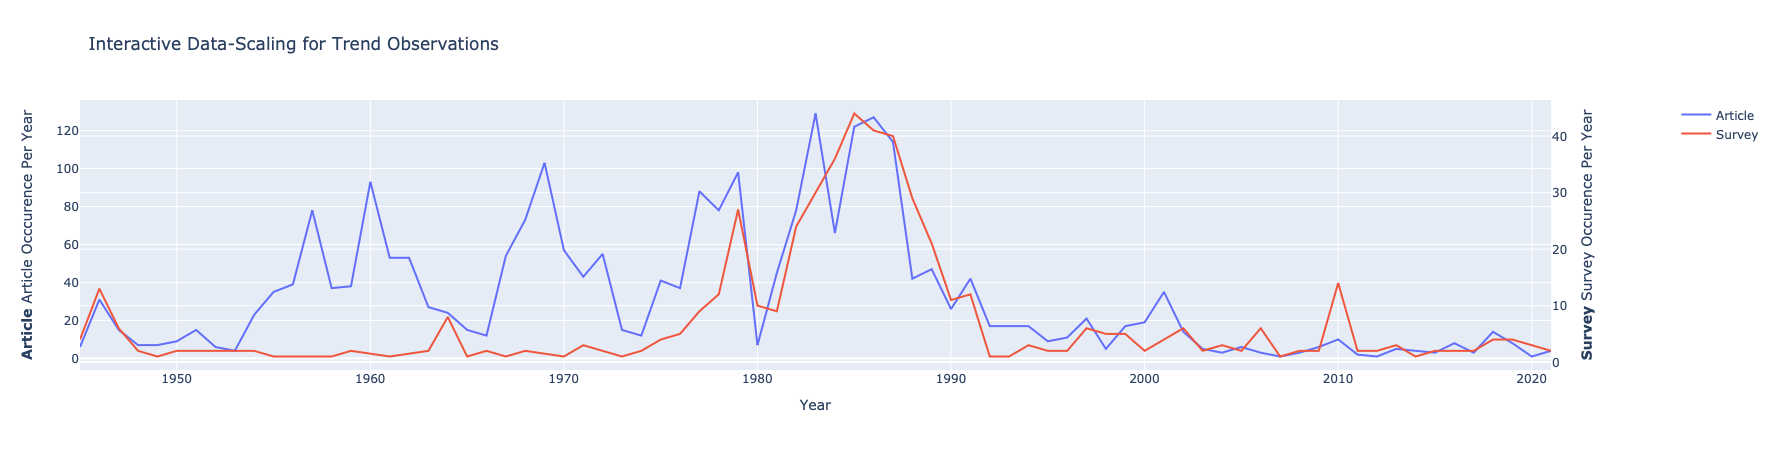
\includegraphics[scale=0.265]{images/Data_Overlay.png}
        \caption{Data-Scaling Comparison by Year}
        \label{fig:Survey Data & Article}
    \end{figure}
    
    Several clear patterns emerge. First, there is a strong correlation between international events and spikes in both media coverage and polling on arms control. When arms control made headlines, it also tended to be the subject of more polling, indicating greater public engagement. For example, the late 1950s to early 1960s show a coincident rise in \textit{NYT} articles (e.g., during the test ban negotiations) and more frequent poll questions about nuclear testing and disarmament \cite{BritannicaNuclearTestBan}. This was a time when policy was moving (LTBT and NPT) and indeed, public opinion and policy were aligned toward progress. The U.S. decision to pursue and sign the LTBT in 1963 matched a period of high public support for banning tests and high media emphasis on arms control’s importance. 
    
    Similarly, the early 1980s freeze movement period shows a peak in media coverage and extensive polling on arms control, reflecting a surge of public sentiment demanding policy action. In that instance, there was partial alignment: while the Reagan administration did not adopt a nuclear freeze, it did enter serious arms reduction talks leading to the INF Treaty, which can be seen as a response consistent with the public’s desire to reduce nuclear dangers. By the late 1980s, when the INF and START I treaties were realized, public opinion was strongly supportive and the policies enacted aligned with public preferences this represents a high watermark of congruence between public will, media advocacy, and policy outcome \cite{TIME1987}. Polls showing 60–80\% approval of treaties like INF and START were matched by successful implementation of those treaties. 
    
    There are also notable cases of misalignment. The case of the Comprehensive Test Ban Treaty in 1999 stands out. In the years leading up to 1999, media coverage of arms control was relatively low (apart from specialist outlets, the CTBT did not dominate news cycles the way Cold War treaties did), and the number of poll questions on arms control in the late 1990s was modest. However, those polls that were conducted found overwhelming support for the CTBT’s goal. The Senate’s rejection of CTBT thus went against public opinion. Why was there not a larger public outcry? One reason may be the lack of sustained media focus without intensive media coverage, the average American might not have been fully aware of the treaty or the implications of its rejection. Indeed, arms control in 1999 did not figure as a major issue in most voters’ minds compared to domestic concerns. This suggests that for public opinion to effectively align with and influence policy, an issue needs both latent support and salience. In CTBT’s case, support was high but salience was low; policymakers under President Clinton failed to rally public attention in a way that could overcome Senate opposition. 
    
    Another misalignment occurred in the late 2010s with the U.S. withdrawal from the INF Treaty (2019) and the near-expiration of New START. Here, media attention to arms control was somewhat higher than earlier in the decade (with many news analyses warning of a new arms race), and polling clearly indicated the public wanted to remain in these agreements. Yet the administration proceeded with withdrawal from INF and was ambivalent about New START (which was ultimately extended in early 2021, just two days before expiration, by a new administration). The INF case is illustrative: two-thirds of Americans in 2019 wanted to stay in the INF Treaty, but the U.S. government withdrew \cite{DefenseOne2019}. This mismatch can be partly explained by the fact that arms control had become a low-salience issue for the public by that point. There were few electoral consequences for withdrawing from INF; the issue was not prominent in campaign debates or likely to sway many votes. Thus, even though the public on balance disagreed with the withdrawal, the intensity of that preference was low, allowing policy to be driven by strategic considerations (concerns about Russia’s violations and China’s missiles, according to officials) rather than public demand. This contrasts with the 1987 INF Treaty’s origin, where public pressure for arms reductions was high, contributing to the treaty’s creation. 
    
    Overall, the data suggest that when public interest and concern about arms control are high, U.S. policy has tended to move in the direction of more arms control (as leaders respond to voters’ desires or at least find public support as a facilitating factor). For instance, public calls for curbing nuclear tests and slowing the arms race helped create a favorable context for the LTBT and NPT in the 1960s and for the freeze movement’s influence on 1980s negotiations. Conversely, when public engagement wanes, arms control can stagnate or even reverse, as seen in the 2000s. The early 2000s withdrawal from the ABM Treaty occurred in a climate where few Americans were focused on missile defense or arms treaties, and indeed there was little public debate. In the comparative sense, media coverage often acts as an intermediary: strong media focus can elevate public salience, which in turn pressures policymakers. The decline of arms control as a headline issue after the Cold War meant fewer feedback loops of this kind. 
    
    However, it is crucial to note that latent support for arms control remained a constant. Even in periods of low media attention, polls show Americans did not turn against arms control agreements—there was no majority clamoring to scrap treaties. Thus, when leadership pursued arms control (like President Obama’s New START in 2010), they had an easy time garnering public approval, even if public demand had not been vocal beforehand. 
    
    We also compare how media-reported views align with direct survey results. In general, \textit{NYT} reporting on arms control often mirrored what polls were indicating. For example, during the debate over the nuclear freeze, \textit{NYT} articles noted the widespread public support for the freeze idea, which matched polling numbers. Media accounts sometimes serve as proxies for public sentiment in the absence of immediate polls. In the 1960s, the \textit{NYT} emphasized the public’s fear of fallout and desire for a test ban, and indeed polling at the time confirmed those sentiments. There were a few instances where media narratives and public opinion appeared misaligned: one could argue the media in 1983–84 was very alarmist about Reagan’s arms buildup and SDI, whereas public opinion still trusted Reagan to handle arms negotiations (as evidenced by his re-election and polls showing confidence in his approach to U.S.–Soviet talks). But by and large, the media did report accurately on public mood – for instance, the 1987 \textit{NYT} coverage of INF’s signing highlighted Midwestern Americans’ relief and support, consistent with the polls showing 62\% approval. 
    
    In terms of alignment with policy decisions, one can identify periods of convergence: the early 1960s, late 1980s, and to an extent the early 2010s (New START) saw public opinion, media support, and policy all pushing in the same direction (toward arms control agreements). Periods of divergence include the early 1980s (initially Reagan’s policy vs public desire for freeze, though this later converged), 1999 (CTBT rejection vs public support), and late 2010s (treaty withdrawals vs public preference to retain treaties). Each divergence has its own explanation, but a common thread is that public support alone is not always enough to carry an arms control policy—political leadership and international conditions matter greatly. 
    
    Conversely, strong public opposition could act as a check on anti-arms-control moves; for example, had there been significant public opposition to leaving the INF Treaty, perhaps the decision might have been more contested. The lack of such opposition can be linked to the reduced salience of arms control in the public’s mind. Indeed, by the 2020s, polls found that issues like infectious disease and terrorism outranked nuclear proliferation as perceived major threats, which may have given policymakers a sense that withdrawing from arms treaties would not hurt them domestically. 
    
    In the final analysis, U.S. arms control policy over the decades has generally enjoyed public backing when it aimed to reduce nuclear risks. Public sentiment has been one of cautious support: Americans typically favor verifiable treaties that mutually limit weapons, and this consensus has been remarkably steady from the Cold War to the present. Media coverage has at times rallied public attention to these issues, reinforcing public pressure for diplomatic solutions. However, when policy decisions have run counter to public opinion (as in the CTBT case or INF withdrawal), it often reflected the fact that public engagement was not acute enough to impose a political cost. The lesson is that alignment between public opinion and policy is strongest when the issue is prominent and the public is activated, whereas in more quiescent periods, policy can diverge from the public’s latent preferences without significant repercussion.


\section{Conclusion}

    This historical analysis demonstrates that American public opinion has been a generally stabilizing force in favor of arms control agreements related to weapons of mass destruction, even as the intensity of that opinion has varied with time. During the Cold War, the terrifying prospect of nuclear conflict forged a public consensus that arms control efforts were necessary; this was reflected in media discourse and in broad support for treaties like the LTBT, NPT, SALT, and INF. That public sentiment often worked in tandem with policy, pushing leaders to negotiate and ratify agreements that reduced nuclear dangers. 
    
    In the post-Cold War era, while the public’s focus shifted to other issues, a baseline support for arms control remained — seen in strong approval for banning chemical weapons, stopping nuclear tests, and extending nuclear arms reduction treaties. When policy aligned with these views, as in the ratification of the CWC in 1997 or New START in 2010, it proceeded with little public controversy. When policy diverged, as in the CTBT rejection or withdrawal from INF, it tended to be a story of political or ideological motivations outweighing an uninspired public rather than a case of public demand for abandoning arms control. 
    
    Media coverage, epitomized by the \textit{New York Times} archive, has both reflected and shaped these opinion trends. In periods of active arms control progress or crisis, the media kept the issue in the spotlight, often highlighting public stakes and sentiment — thereby creating a feedback loop that bolstered policy action. In quieter times, media attention waned, and arms control fell off the public agenda, giving policymakers more autonomy to act (or not act) without electoral imperatives. 
    
    In conclusion, the alignment between U.S. public opinion and arms control policy has been strongest when the dangers of WMD were salient and immediate, prompting public outcries for action that translated into diplomatic outcomes. Public sentiment shifts in response to events — rising anxiety during arms races or after near-miss crises leading to greater support for agreements, and complacency during calmer periods leading to less pressure on leaders. Yet throughout these fluctuations, the American public’s fundamental predisposition has leaned toward favoring arms control measures as instruments to enhance security. This enduring predisposition means that even if arms control is not always a top-tier issue, there exists a reservoir of public goodwill toward efforts that limit WMD threats. Policymakers who have tapped into that reservoir, working with media to inform and engage the public, have generally found success in aligning national policy with the public interest in reducing the specter of mass destruction. Conversely, when arms control has stagnated or regressed, it has often been when that connection to public sentiment was weak or neglected.  
    
    In the face of future challenges — from nuclear modernization and new technologies to multipolar arms competition — understanding this historical interplay between public opinion and arms control policy is crucial. It suggests that revitalizing public engagement on arms control could be key to advancing new agreements. If leaders clearly communicate the stakes and the benefits of arms control, the latent support among Americans could be reactivated, influencing policy choices toward restraint and international cooperation \cite{GlobalAffairs2017}. History shows that when the American public is engaged and supportive, it provides a strong mandate for arms control initiatives; when disengaged, opportunities for arms control may be lost. The past thus provides both a reassurance that public appetite for reducing WMD dangers persists, and a caution that maintaining alignment with that appetite requires effort in public discourse.
    

\cite{ArmsControlColdWar}\cite{BritannicaLTBT}\cite{Carnegie1999}\cite{CDI2002}\cite{ArmsControlColdWar}\cite{ChicagoCouncil2017}\cite{Graham1989}\cite{FifthEstate1982}


\section{Acknowledgements}

    This research was supported by provisional access to the New York Times Archive API for research purposes.
    
    This research was supported by provisional access to the iRoper polling database through an institutional agreement.


\newpage

\printbibliography

\end{document}

